\chapter{Scope}
In this project, the scope of the research is of extreme relevance. Given the fact that the problem identified and the main research question are general, the scope will contribute to stress the focus and delimit those domains that are beyond the current project.\par
This dissertation will take a quantitative approach to study the urban systems and develop digital tools. Approaching the research questions stated above, immediately reduces the scope of this work, specially as it will become clearer below, when these ideas are intersected with the ideas of circular economy.\par



\begin{figure}[h!]
    \centering
    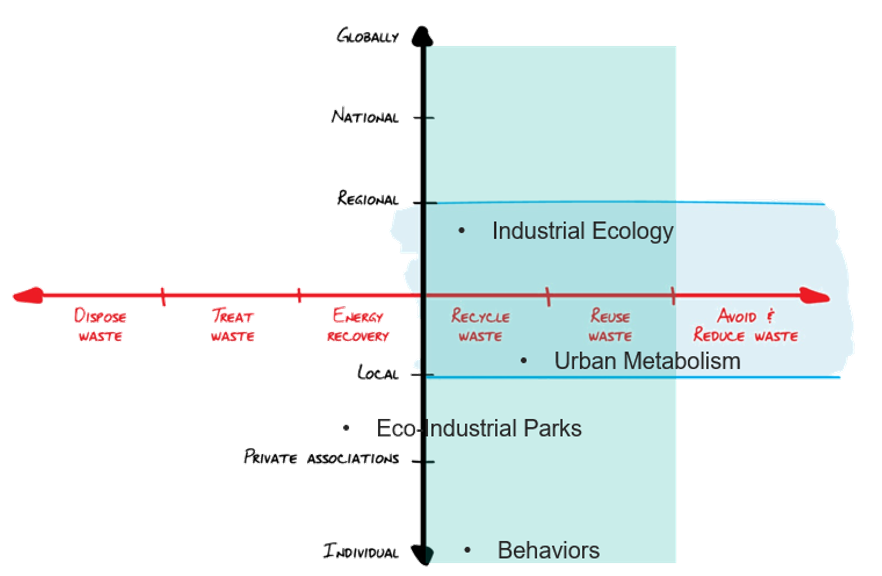
\includegraphics[width=0.8\textwidth]{sections/asset/scopeee.PNG}
    \caption{Scope of the research}
    \label{fig:scope}
\end{figure}



\section{Type of research}
In order to delimit this project and to position this research in terms of the ecosystem of the work done about Circular Economy, the review done by \textcite{Merli2018} is used. In this work different academic articles working with Circular Economy are studied and different categories are suggested. This work is of importance since, it provides a general knowledge of the type of research that is being done and how Circular Economy is approached. In the following table, extracted from this article, different structural dimensions are presented. Each domain contains different analytical categories which are used to study the concept. 

\begin{figure}[h!]
    \centering
    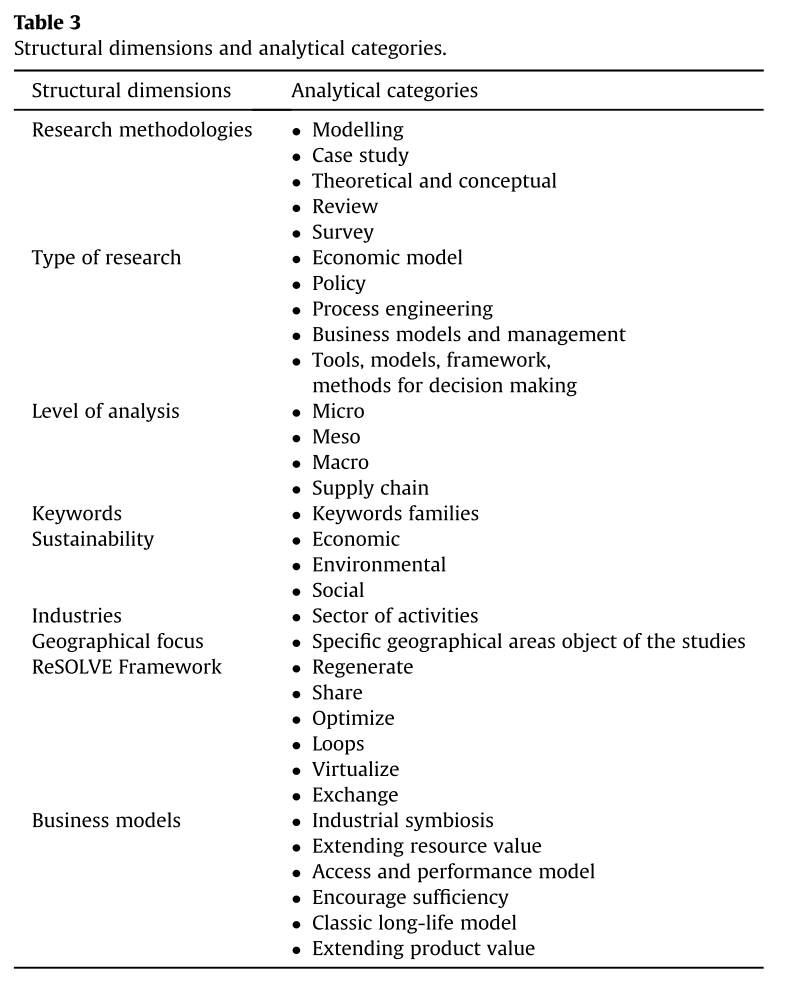
\includegraphics[width=0.6\textwidth]{sections/asset/cateogories of research.PNG}
    \caption{Categories of research}
    \label{fig:research cat}
\end{figure}

Regarding the different research methodologies, as analytical tools this research will be focusing on building conceptual frameworks, that can be used to model and take case studies to test the models. This means, that the type of research that will be engaged in this project will be aimed to develop tools, models, framework and/or methods for decision making. \par

Since the objective is to develop a general model to capture how waste flows in city-regions, this automatically means that the levels of analysis and scale of the project will be somewhere between a meso and macro level. Here individual choices or behavioral characteristics will be not be explored. \par
Finally, it will be focus on waste exchanges of different kinds, trying to understand to what extent the location of socio-economic activities affect the level of Circular Economy practices. 




\section{Circular Economy}

The research on CE is still at early stages and the role of location socio-economic activities within it needs to be further researched. As UN, EU and other governments as China, Singapore, Japan or The Netherlands, to name a few, make efforts to transition towards circular economy models, the paradigm/concept has expanded to city planning (Circular Cities, XXXXXX). Among the different circular economy strategies, in solid waste management and industrial symbiosis there are geographical elements to be considered and consequently of relevance for spatial planning agencies.\par

In this exploratory research project these different CE strategies will be approached with different objectives and methods; hoping that by making contributions and reflecting on these individual fields a more general statement about the relevance of planning can be made.\par

Dealing with IS and SWM, automatically creates another exclusion in the concept of CE. As the concept of CE could be found rooted as a spin of the 3Rs strategy to reduce the amount of waste produced (Reduce-Reuse-Recycle). Since its first appearance the idea of 3Rs has evolved and more Rs and other letters have been added to the main idea. Currently, the concept has crystallized into a 6 stages pyramid and this work will focus in the 2 stages of it: recycle waste, reuse waste. \par



\section{Geographical considerations}
Because of the geographical nature of Circular Economy, the work will be focused on SWM and IS and these systems cannot be contained to cities administrative boundaries \parencite{Dupuy2008}. The production of waste resources and it’s treatment are scattered across the territory, with interactions across municipalities and in some cases regions, thus require to take a more holistic and comprehensive approach. \par
Although, the exploration of theses strategies could be done under different scales; starting from an individual stakeholder, moving upwards in scale to a group, a neighbourhood a city and the system of cities that comprehend the system, in order to comprehend how sustainable the system is, it's important to take into consideration not only one unit but the whole network of cities that create a functional area.\par 




\section{Approach/Methodological}
The work developed during this project will be quantitative and embraces the Smart Cities movement. The work will benefit from advances in computer science, new sources of information and urban analytics. This delimitation is important because it defines the lenses and toolkit used to analyze the problem of waste materials in city regions. \par
The planning tools and frameworks of this works, need to be digital and with the capacity of capturing in a quantitative matter the dynamics of the system.\par
Moreover, an open-source and full transparency approach will be also adopted. This is an important condition of the present work because it will allow other researchers and practitioners to understand the tool box to be developed, but also by adopting this paradigm it allows the project to continue after it finishes. Everyone interested in improving or correcting these developments will be able to do it.  


\section{Other research delimitation}
Arguably, Circular Economy can be considered the next new paradigm that will contribute to materialize sustainable development. In order to qualify as such, the contribution to the three main sustainable development domains (Economically, Social \& Environmental) should become clearer. %(xxxxxxx). 
Research on CE is still in its infant stages and the concept is found contested.  %(XXXXX). 
Variations in its definition makes it difficult to implement creating gaps between theory and practice. \par %(XXXXXXX). \par

In this work, CE is understood as a set of strategies that eventually could became a new socio-economic regime but the contributions of ce to promote social justice are still unexplored. Moreover, issues related to institutions, politics or even behavioral changes such as trust or citizen involvement are out of the scope of the dissertation.\par
Finally, but not least important it is important to state that within the field of IS there is a an already well-developed corpus of research that focuses in Eco-Industrial Parks (EIP), which are co-located firms in pre-determined zone. Usually in these types of industrial developments, there is a natural tendency to reduce energy, water and other resources. Also, as a result of lower barriers IS arriving to higher stages of development: knowledge exchanges and other forms of co-operation. \par



\section{Case Studies}
Finally, the general framework and data model developed during this project are going to be tested by applying it to different context. For it, data availability will be crucial. This will require to establish relationships with different stakeholders and to begin a collaboration process. Currently, there are some potential institutions to collaborate with that work in the following places:
\begin{enumerate}
    \item CEAMSE - Buenos Aires Metropolitan Area
    \item WET - Sweden
    \item Metabolic - Netherlands
\end{enumerate}




%\section{Summary}

%This is an exploratory dissertation that will be trying to make a quantitative contribution to understand how space can be taken into consideration to enhance circular economy practices. In order to do so, among the different strategies 



